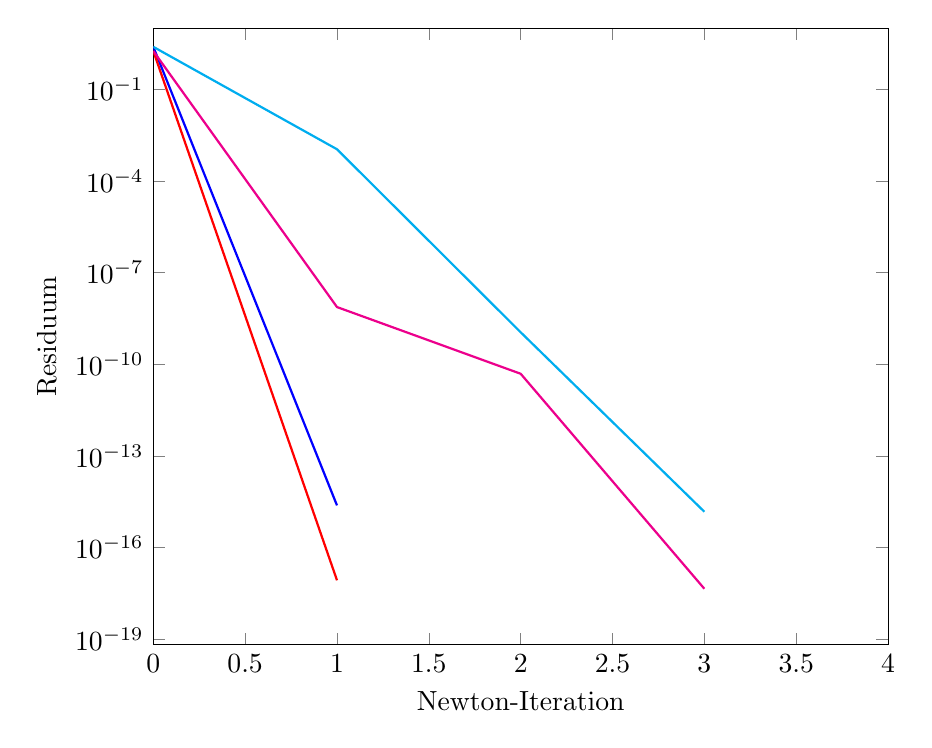
\begin{tikzpicture}[every plot/.append style={thick}] 
\begin{axis}[ 
label style={font=\normalsize}, 
xlabel={Newton-Iteration}, 
ylabel={Residuum}, 
xmin=0, xmax=4, 
ymode=log, 
ymin=0, ymax=10, 
width=0.9\textwidth, 
grid style=dashed, 
] 
\addplot[ 
color=blue, 
] 
coordinates { 
(0, 2.46e+00)(1, 2.39e-15)}; 
\addplot[ 
color=red, 
] 
coordinates { 
(0, 1.79e+00)(1, 8.45e-18)}; 
\addplot[ 
color=cyan, 
] 
coordinates { 
(0, 2.46e+00)(1, 1.09e-03)(2, 1.11e-09)(3, 1.48e-15)}; 
\addplot[ 
color=magenta, 
] 
coordinates { 
(0, 1.79e+00)(1, 7.44e-09)(2, 4.87e-11)(3, 4.45e-18)}; 
\end{axis} 
\end{tikzpicture} 
